\subsection{Calorimetry system}
%The detector systems downstream of \richtwo, namely the muon and calorimetry systems, are used for
%\pid and in the trigger; triggering will be covered in the following section.
%As discussed, the \rich detectors excel in hadron identification; for the identification of
%electrons, photons and muons information from the five muon stations (M1-5) and calorimetry system
%are used.
%The calorimeters are situated between M1 and M2--5.

The general structure of the calorimetry system is that of an \ecal followed by an \hcal, but
before both these stations there are additional calorimetry systems designed to provide some \pid
in the trigger; this is discussed later.
The primary function of the calorimetry system is for triggering high \pt hadrons, electrons and
photons --- this is described in detail in \Sec{sec:lhcb:trig}.

The \spd is positioned just downstream of M1, which in turn is immediately downstream of \richtwo
and set apart from the other muon stations M2--4.
The \spd is made of scintillating tiles which detect charged particles, and therefore can be used
to distinguish electrons from photons.
Following the \spd is a $15\mm$, $2.5\,X_0$, thick lead plate followed by the \presh detector,
whose design is almost identical to the \spd.
The \presh exploits the showering caused by the lead plate to distinguish between electromagnetic
particles and hadrons.

The \ecal is a shashlik detector, made of alternating layers of lead, reflector, and scintillating
material.
Light from the scintillators is guided to photomultiplier tubes by wavelength shifting fibres.
This \ecal subdetector is 25 radiation lengths long,  ensuring that all electromagnetic energy is
deposited before the \hcal.
The energy resolution of the \ecal is
\begin{equation}
  \frac{\sigma_E}{E} = \frac{10\pc}{\sqrt{E}} \oplus 1\pc,
\end{equation}
where $E$ is in GeV.

Figure~\ref{fig:lhcb:calo} shows the difference in geometry between the \ecal and \hcal.
The \hcal also has a shashlik design (where the scintillators are interleaved with iron), but where
the faces of the tiles in the \ecal are oriented
towards the incoming particle flux, the \hcal tiles are oriented longitudinally.
Each subdetector within the calorimetry system has increased cell density near the beam to cope
with higher track multiplicity in this region
Due to restrictions in space, the \hcal is only 5.6 nuclear interaction lengths long and has a
resolution of
\begin{equation}
  \frac{\sigma_E}{E} = \frac{(69\pm5)\pc}{\sqrt{E}} \oplus (9\pm2)\pc,
\end{equation}
where $E$ is in GeV.
% trigger does not need full shower containment, so optimized for space

\begin{figure}
  \begin{center}
    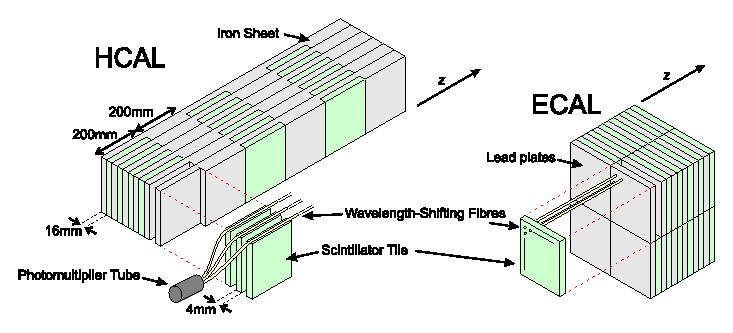
\includegraphics[width=0.98\textwidth]{calo_structure.pdf}
    \caption[The LHCb calorimeters]
    {\small
      Geometry of the \lhcb \hcal and \ecal.
    }
    \label{fig:lhcb:calo}
  \end{center}
\end{figure}

